\documentclass[11pt]{article}


\usepackage[sort]{natbib}
\usepackage{bm,amsmath,bbm,amsfonts,nicefrac,latexsym,amsmath,amsfonts,amsbsy,amscd,amsxtra,amsgen,amsopn,bbm,amsthm,amssymb,graphicx}
\usepackage{fancyhdr}
\usepackage[margin=1.0in]{geometry}




\title{Second Monitoring Committee Meeting\\\vspace{4mm} \normalsize{Understanding the information content in diverse observations of forest carbon stocks and fluxes for data assimilation and ecological modelling.}}
\date{\normalsize{16$^{th}$ May 2014, \ Room TBC}}
\author{\normalsize{E. Pinnington}}


\newtheorem{theorem}{Theorem}[section]
\newtheorem*{defn}{Definition}



	
\begin{document}

\maketitle

\section*{Project Background}

A large amount of data is currently being gathered that is relevant to the carbon balance of forests, with much of this data coming from Eddy covariance flux towers \cite{baldocchi2008turner}. Attempts are also being made to combine this data with models of forest carbon stocks and fluxes, such as the Data Assimilation Linked Ecosystem Carbon model (DALEC) \cite{williams2005improved}, in a data assimilation (DA) scheme. Currently, however, there are limitations with such schemes as there is a lack of understanding about the additional information provided by different observations. Current DA schemes for ecosystem carbon flux only specify the diagonal elements of the observation error covariance matrix, $\textbf{R}$, which correspond to the individual uncertainties in particular observations. As such, these DA schemes do not specify observation error correlations or covariances, corresponding to the off diagonal elements of $\textbf{R}$. In numerical weather prediction (NWP) it has been shown that the inclusion of observation error correlations can increase the information content from a given data set and reduce analysis error \cite{stewart2008correlated}. Better understanding the information content and error correlations of carbon balance observations will form one of the main aims of the project.

\section*{The DALEC model}

The DALEC model is a simple process-based model describing the carbon balance of an evergreen forest ecosystem. The model is constructed of five carbon pools (foliage ($C_f$), fine roots ($C_r$), woody stems and coarse roots ($C_w$), fresh leaf and fine root litter ($C_l$) and soil organic matter and coarse woody debris ($C_s$)) linked via fluxes. The gross primary production function ($GPP$) uses meteorological driving data and the site's leaf area index (a function of $C_f$) to calculate the total amount of carbon to be allocated at a daily time step.   
\begin{figure}[h!]
    \centering
    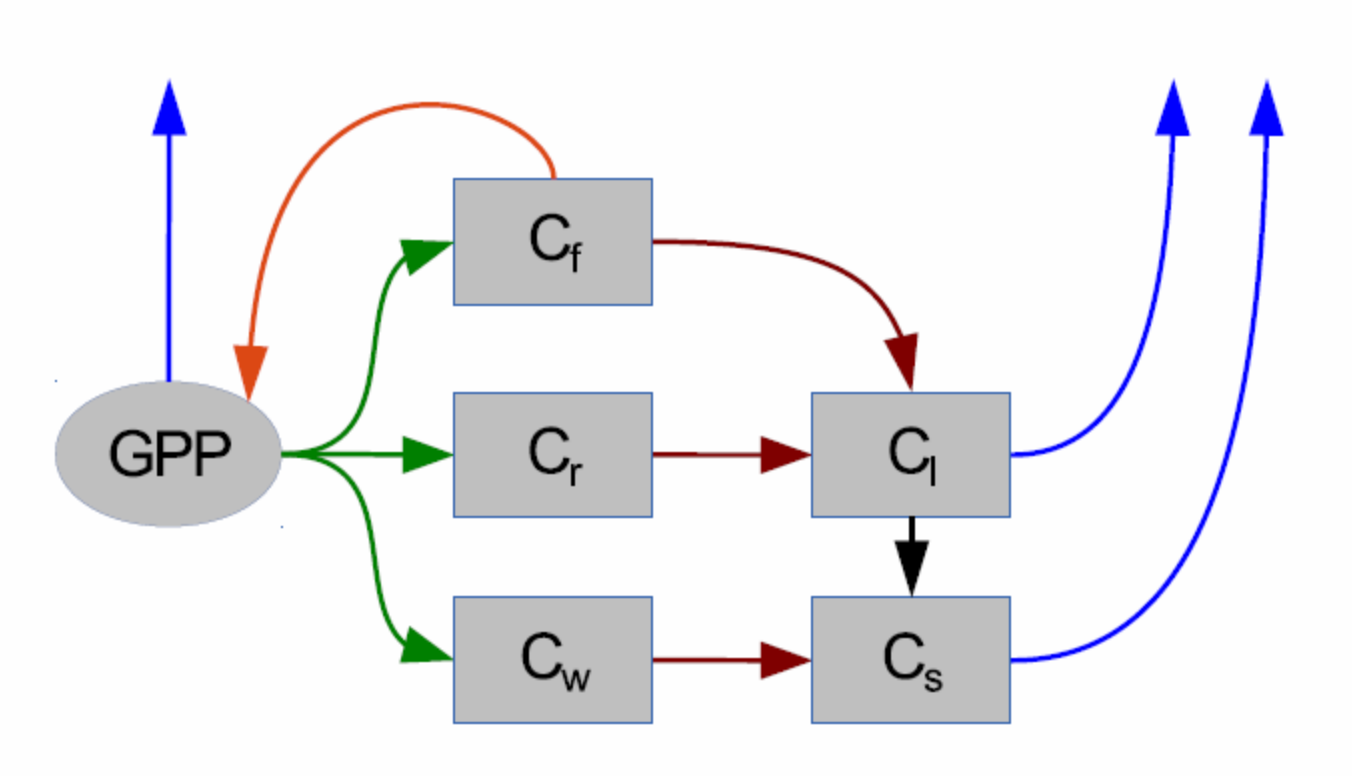
\includegraphics[width=0.5\textwidth]{DALECpic.png}
    \caption{DALEC carbon balance model \cite{delahaies2013regularization}}
    \label{fig:DALEC_mod}
\end{figure}
The model equations for the carbon pools at day $t+1$ are as follows:
\begin{align*}
C_f(t+1)&=(1-p_5)C_f(t)+p_3(1-p_2)GPP(C_f(t),\phi),
\\C_r(t+1)&=(1-p_7)C_r(t)+p_4(1-p_3)(1-p_2)GPP(C_f(t),\phi), 
\\C_w(t+1)&=(1-p_6)C_w(t)+(1-p_4)(1-p_3)(1-p_2)GPP(C_f(t),\phi), 
\\C_l(t+1)&=(1-(p_1+p_8)T(t))C_l(t)+p_5C_f(t)+p_7C_r(t), 
\\C_s(t+1)&=(1-p_9T(t))C_s+p_6C_w(t)+p_1T(t)C_l(t).
\end{align*}
Where $T(t)=\frac{1}{2}exp(p_{10}T_m(t))$, $T_m$ is daily mean temperature, $p_1,\ldots,p_{10}$ are rate parameters and $\phi$ represents the meteorological driving data used in the $GPP$ function. The full details of this version of DALEC can be found in \cite{williams2005improved}.

\section*{Shannon Information Content and Observation Sensitivity}

In DA Shannon Information Content ($SIC$) is a measure of the reduction in entropy given a set of observations. Entropy physically corresponds to the volume in state space taken up by the probability density function (pdf) describing the knowledge of the state \cite{rodgers2000inverse}. Assuming all pdfs are Gaussian we have,
\[
SIC=\frac{1}{2}ln\frac{\begin{vmatrix} \bf{B} \end{vmatrix}}{\begin{vmatrix} \bf{A} \end{vmatrix}}
\]
where $\bf{B}$ is the background error covariance matrix and $\bf{A}$ is the analysis error covariance matrix. For a larger reduction in uncertainty in our analysis we have a larger value of $SIC$. I began by using $SIC$ to understand the information content for different sets of observations at one time when being assimilated with the DALEC model, specifying the state vector for the assimilation as,
\[ \underline{x}_b = (C_f, C_r, C_w, C_l, C_s)^T. \] 
Where the elements of the state vector have variances, $\sigma_{cf,b}^{2},\ldots,\sigma_{cs,b}^{2}$, respectively. Giving a background error covariance,
\[
\bf{B} = \begin{pmatrix} 
\sigma_{cf,b}^{2} & 0 & 0 & 0 & 0 \\
0 & \sigma_{cr,b}^{2} & 0 & 0 & 0 \\
0 & 0 & \sigma_{cw,b}^{2} & 0 & 0 \\
0 & 0 & 0 & \sigma_{cl,b}^{2} & 0 \\
0 & 0 & 0 & 0 & \sigma_{cs,b}^{2} \\
\end{pmatrix}.
\]  
Here I have assumed a diagonal background error covariance matrix. For $\textbf{A}^{-1}$ we have,
\[
\textbf{A}^{-1}=\textbf{J}'' = \textbf{B}^{-1}+\textbf{H}^{T}\textbf{R}^{-1}\bf{H}. 
\]
Where $\textbf{J}''$ is the Hessian of $\bf{J}$, the cost function to be minimized in Three-Dimensional Variational Data Assimilation (3D-Var), and $\bf{H}$ is the linearized observation operator. One of the main observations made of forest carbon balance at flux tower sites is the net ecosystem exchange ($NEE$) of CO$_{2}$ which can be estimated by DALEC as the difference between $GPP$ and the respiration's of $C_l$ and $C_s$ giving,
\[ 
NEE(t)=(1-p_2)GPP(C_f(t),\phi)+p_8C_lT(t)+p_9C_sT(t). 
\]
For a single observation of $NEE$ at one time, $t_0$, an analytical expression for the $SIC$ can be derived using,
\[
\textbf{H}_{0} = \begin{pmatrix}
(1-p_{2})\zeta_0 & 0 & 0 & p_{8}T_{0} & p_{9}T_{0}
\end{pmatrix},
\]  
where $\zeta_0 = GPP'(C_f(t_0), \phi)$, $T_{0}=T(t_0)$ and $\textbf{H}_{0}$ is the linearized observation operator at time $t_0$. As we have a single observation at one time our observation error covariance matrix, $\bf{R}$, is just the variance of our observation of $NEE$, $\sigma_{nee,0}^{2}$, at time $t_0$. So that,
\[
\textbf{R}=\sigma_{nee,0}^{2}
\]  
and
\[
\begin{array} {lcl}
\textbf{J}'' &=& \textbf{B}^{-1}+\textbf{H}^{T}\textbf{R}^{-1}\bf{H} \\
&=& \begin{pmatrix} 
\sigma_{cf,b}^{-2}+\sigma_{nee,0}^{-2}(1-p_{2})^{2}\zeta_0^{2} & 0 & 0 & \sigma_{nee,0}^{-2}(1-p_{2})\zeta_0 p_{8}T_0 & \sigma_{nee,0}^{-2}(1-p_{2})\zeta_0 p_{9}T_0 \\
0 & \sigma_{cr,b}^{-2} & 0 & 0 & 0 \\
0 & 0 & \sigma_{cw,b}^{-2} & 0 & 0 \\
\sigma_{nee,0}^{-2}(1-p_{2})\zeta_0 p_{8}T_0 & 0 & 0 & \sigma_{cl,b}^{-2}+\sigma_{nee,0}^{-2}p_{8}^2 T_0^2 & \sigma_{nee,0}^{-2}p_{8}p_{9} T_0^2 \\
\sigma_{nee,0}^{-2}(1-p_{2})\zeta_0 p_{9}T_0 & 0 & 0 & \sigma_{nee,0}^{-2}p_{8}p_{9} T_0^2 & \sigma_{cs,b}^{-2}+\sigma_{nee,0}^{-2}p_{9}^2 T_0^2 \\
\end{pmatrix}.
\end{array}
\] 
We then have,
\[
SIC=\frac{1}{2}ln\frac{\begin{vmatrix} \textbf{B} \end{vmatrix}}{\begin{vmatrix} \textbf{A} \end{vmatrix}} = \frac{1}{2}ln\begin{vmatrix} \textbf{B} \end{vmatrix}\begin{vmatrix} \textbf{J}'' \end{vmatrix}.
\]
So that,
\[
SIC = \frac{1}{2}ln\frac{(p_{2}-1)^{2}\zeta_0^{2}\sigma_{cf,b}^{2}+\sigma_{nee,0}^{2}+T_{0}^2(p_{9}^2\sigma_{cs,b}^2+p_8^2\sigma_{cl,b}^2)}{\sigma_{nee,0}^{2}}.
\]
If we assume that the variances and parameters here are fixed we can see that the size of the $SIC$ is dependent on the temperature term, $T_0$, and the square of the first derivative of $GPP$, $\zeta_0^{2}$. Generally the value of $GPP$ (and its first derivative) is highest in summer with higher total daily irradiance and higher temperatures. We therefore have that there will be more information content in observations that are taken when temperatures are higher. I have also derived analytical forms for the $SIC$ using different sets of observations at a single time which all have a similar form.

Following this work based at a single time I started looking at the $SIC$ when successive observations are added over a period of time. The model was now built into a Four-Dimensional Variational Data Assimilation (4D-Var) framework where our observation operator, $\textbf{H}$, and observation error covariance matrix, $\textbf{R}$, are now,
\[ 
\textbf{H}=
\begin{pmatrix}
\textbf{H}_0 \\
\textbf{H}_1\textbf{M}_0\\
\vdots \\
\textbf{H}_n\textbf{M}_{n,0}
\end{pmatrix}
\hspace{5mm} \text{and} \hspace{5mm}
\textbf{R}=
\begin{pmatrix}
\textbf{R}_0 & 0 & 0 & 0 \\
0 & \textbf{R}_1 & 0 & 0 \\
0 & 0 & \ddots & 0 \\
0 & 0 & 0 & \textbf{R}_n
\end{pmatrix}.
\]
Where $\textbf{H}_i$ is our linearized observation operator at time $t_i$, $\textbf{M}_{i,0}=\textbf{M}_{i-1}\textbf{M}_{i-2}\cdots\textbf{M}_0$ is our linearized model evolving the state vector, $\underline{x}_b$, at time $t_0$ to time $t_i$ and $\textbf{R}_i$ is the observation error covariance matrix corresponding to $\textbf{H}_i$ at time $t_i$ \cite{lewis2006dynamic}. I first calculated the adjoint model for DALEC analytically as $\textbf{M}_i=\frac{\delta \underline{m}_i}{\delta \underline{x}_i}$. I then wrote a code in Python that calculates $\textbf{H}$ and $\textbf{R}$ to find a value of $SIC$ when successive observations of $NEE$ are made each day over a chosen period (To calculate the $SIC$ we do not need the actual observation value). The meteorological driving data used in the model is taken from a ponderosa pine forest in central Oregon for which the DALEC model in \cite{williams2005improved} is parameterized. Below we have a plot when different starting points and periods are chosen, day 0 represents the start of the year so that day 200 is during the summer,
\begin{figure}[h!]
\centering
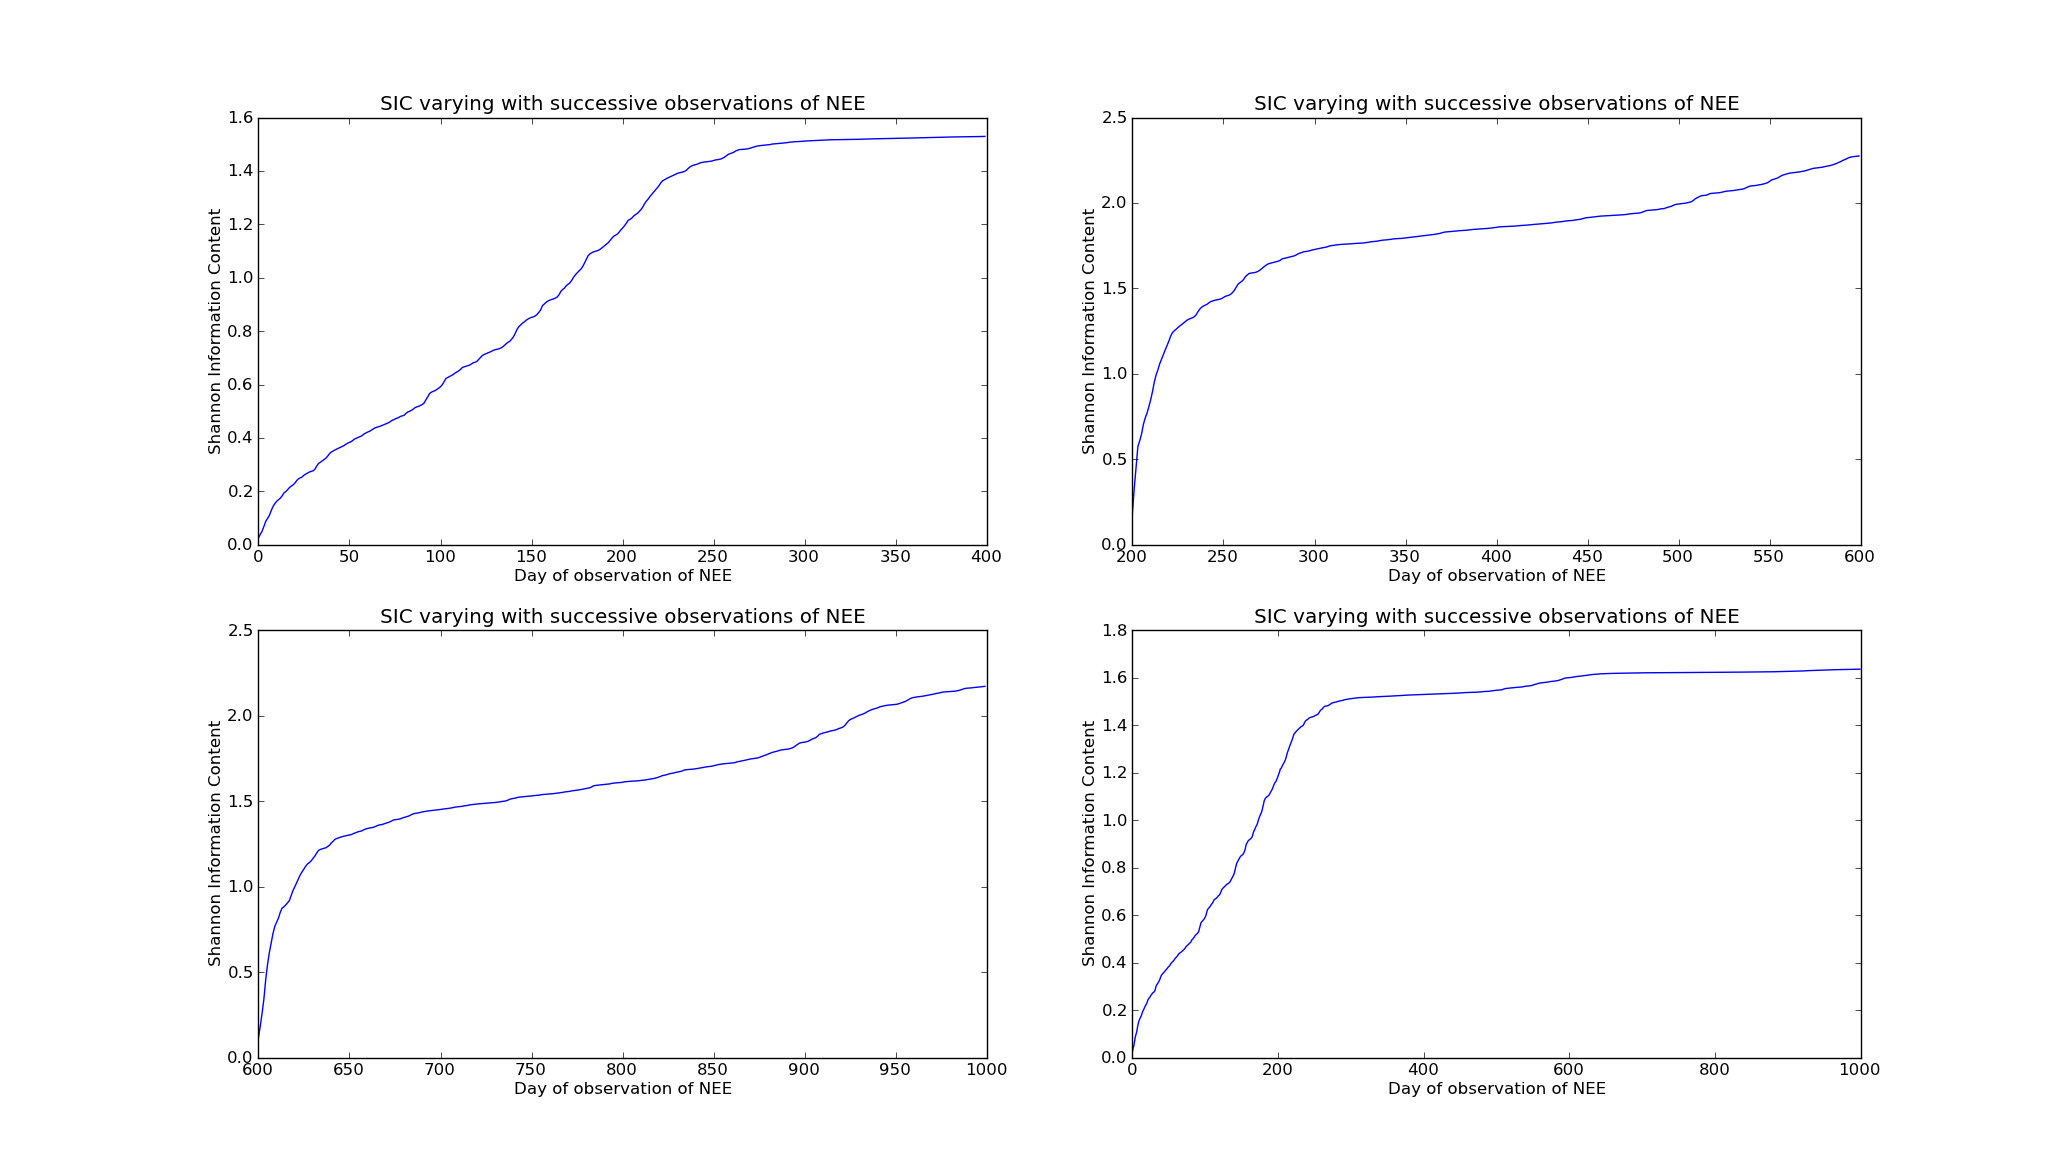
\includegraphics[width=1\textwidth]{SICsubplot.png}
\caption{$SIC$ varying as successive observations of $NEE$ are added using driving data from Oregon pine forest.}
\label{fig:SIC_subplot}
\end{figure}





\bibliography{../../PhD}{}
\bibliographystyle{plain}
\end{document}
